%%% user_manual.tex --- 

%% Author: XX.YY@IDEALX.com
%% Version: $Id$

\def\RCS$#1: #2 ${\expandafter\def\csname RCS#1\endcsname{#2}}
\RCS$Revision$
\RCS$Date$

\documentclass{IDXDOC-en}
\usepackage{idx-shortcuts}

% --------------------------------------------
% Title 
% --------------------------------------------
\doctitle{IDX-Tsunami User's manual}

%\addauthor{Nicolas}{Niclausse}{nicolas.niclausse@IDEALX.com}

\doccopyright{IDEALX S.A.S.}
\docversion{\RCSRevision}
\docreldate{\RCSDate}
\docref{idx-tsunami-user-manual}

\begin{document}
\maketitle
\Abstract{IDX-Tsunami user's manual}
\newpage
\tableofcontents

\section{Introduction}

\subsection{What is IDX-Tsunami ?}

\program{IDX-Tsunami} is a distributed load testing tool. It is
protocol-independent and can currently be used to stress HTTP, SOAP
and Jabber servers.

It is distributed under the GNU General Public License version 2.

\subsection{What is Erlang and why is it important for IDX-Tsunami ?}

\program{IDX-Tsunami} main strength is its ability to simulate a huge number a
simultaneous user from a single CPU. When used on cluster you can
generate a really impressive load on a server with a modest cluster,
easy to set-up and to maintain.

\program{IDX-Tsunami} is developed in Erlang and this is where the power
of \program{IDX-Tsunami} relies.

\par Erlang is a \emph{concurrency-oriented} programming language.
Tsunami is based on the Erlang OTP (Open Transaction Platform) and
inherits several characteristics from Erlang: 

\begin{itemize}
\item \emph{Performance}: Erlang has been made to support hundred thousands
of lightweight processes in a single virtual machine. 
\item \emph{Scalability}: Erlang development environment is naturally
distributed, promoting the idea of process's location transparency. 
\item \emph{Fault-tolerance}:Erlang has been built to develop robust,
fault-tolerant systems. As such, wrong answer sent from the server
to \program{IDX-Tsunami} does not make the whole running benchmark crash. 
\end{itemize}

More informations on Erlang on \url{http://www.erlang.org} and
\url{http://www.erlang-projects.org/}


\subsection{IDX-Tsunami background}

History:
\begin{itemize}
\item \program{IDX-Tsunami} is being developed since 2001 
\item It is an industrial implementation of a \emph{stochastic model}
for real users simulation. User events distribution is based on a
Poisson Process. More information on this topic in:

Z. Liu, N. Niclausse, et C. Jalpa-Villanueva.  \strong{Traffic Model
  and Performance Evaluation of Web Servers}. \emph{Performance Evaluation,
Volume 46, Issue 2-3, October 2001}.

\item This model has already been tested in the INRIA \emph{WAGON}
  research prototype (Web trAffic GeneratOr and beNchmark). WAGON was
  used in the \url{http://www.vthd.org/} project (Very High Broadband
  IP/WDM test platform for new generation Internet applications, 2000-2004).

\end{itemize}

\program{IDX-Tsunami} has been used for very high load tests:
 
\begin{itemize}
\item \emph{Jabber} protocol: 10 000 simultaneous users.
  \program{IDX-Tsunami} were running on a 3-computers cluster (CPU
  800Mhz)
\item \emph{HTTP and HTTPS} protocol: 12 000 simultaneous users.
  \program{IDX-Tsunami} were running on a 4-computers cluster. The
  tested platform reached 3 000 requests per second.
\end{itemize}

\program{IDX-Tsunami} has been used  at: 

\begin{itemize}
\item \emph{DGI} (Direction G�n�rale des imp�ts): French finance ministry 
\item \emph{Cap Gemini Ernst \& Young}
\item \emph{IFP} (Institut Fran�ais du P�trole): French Research Organization
for Petroleum 
\item \emph{LibertySurf}
\end{itemize}

\section{Features}

\subsection{IDX-Tsunami main features}

\begin{itemize}
\item \emph{High Performance}: \program{IDX-Tsunami} can simulate a
  huge number of simultaneous users par physical computer: It can
  simulates thousands of users on a single CPU (Note: a simulated user
  is not always active: it can be idle during a \varname{thinktime}
  period). Traditional injection tools can hardly go further than a
  few hundreds (Hint: if all you want to do is requesting a single URL
  in a loop, use \program{ab}; but if you want to build complex
  scenarios with extended reports, \program{IDX-Tsunami} is for you).
\item \emph{Distributed}: the load can be distributed on a cluster of
client machines 
\item \emph{Multi-Protocols} using a plug-in system: HTTP (both standard
web traffic and SOAP) and Jabber are currently supported. LDAP and
SMTP are on the TODO list. 
\item \emph{SSL} support 
\item \emph{Several IP addresses} can be used on a single machine using
the underlying OS IP Aliasing 
\item \emph{OS monitoring} (CPU, memory and network traffic) using Erlang
agents on remote servers or \emph{SNMP}
\item \emph{XML configuration system}: complex user's scenarios are written
  in XML. Scenarios can be written with a simple browser using the
  tsunami recorder (for HTTP only).
\item \emph{Dynamic scenarios}: You can get dynamic data from the
  server under load (without writing any code) and reinject it in
  subsequent requests.
\item \emph{Mixed behaviours}: several sessions can be used to simulate
different type of users during the same benchmark. You can define
the proportion of the various behaviours in the benchmark scenario. 
\item \emph{Stochastic processes}: in order to generate a realistic traffic,
user thinktimes and the arrival rate can be randomize using a probability
distribution (exponential currently) 
\end{itemize}

\subsection{HTTP related features}

\par 


\begin{itemize}
\item HTTP/1.0 and HTTP/1.1 support
\item GET and POST requests 
\item Cookies: Automatic cookies management 
\item \verb|'|GET If-modified since\verb|'| type of request 
\item WWW-authentication Basic 
\item Proxy mode to record sessions using a Web browser 
\item SOAP support using the HTTP mode (the SOAPAction HTTP header is
  handled).
\item HTTP server or proxy server load testing.
\end{itemize}

\subsection{Jabber related features}

\begin{itemize}
\item Authentication, presence and register messages 
\item Chat messages to online or offline users 
\item Roster set and get requests 
\item Global users\verb|'| synchronization can be set on specific actions
\item raw XML messages
\end{itemize}

\subsection{Complete reports set}

Measures and statistics produced by Tsunami are extremely feature-full.
They are all represented as a graphic. \program{IDX-Tsunami} produces
statistics regarding:

\begin{itemize}
\item \emph{Performance}: response time, connection time, decomposition
of the user scenario based on request grouping instruction (called \textit{transactions}), requests
per second 
\item \emph{Errors}: Statistics on page return code to trace errors 
\item \emph{Target server behaviour}: An Erlang agent can gather information
from the target server(s). Tsunami produce graphs for CPU and memory
consumption and network traffic. SNMP is also supported. 
\end{itemize}
\par Note that \program{IDX-Tsunami} take care of the synchronization process
by itself. Gathered statistics are �synchronized�.

 It is possible to generate graphs during the benchmark as statistics
are gathered in real-time.

\subsection{Highlights}

\program{IDX-Tsunami} has several advantages over other injection tools: 


\begin{itemize}
\item \emph{High performance} and \emph{distributed benchmark}: You
  can use IDX-Tsunami to simulate tens of thousands of virtual users.
\item \emph{Ease of use}: The hard work is already done for all supported
protocol. No need to write complex scripts. Dynamic scenarios only
requires small trivial piece of code.
% Tsunami scenarii realisation is mostly based on 
\item \emph{Multi-protocol support}: \program{IDX-Tsunami} is for example one of
the only tool to benchmark SOAP applications 
\item \emph{Monitoring} of the target server(s) to analyze the behaviour
and find bottlenecks. For example, it has been used to analyze cluster
symmetry (is the load properly balanced ?) and to determine the best
combination of machines on the three cluster tiers (Web engine, EJB
engine and database) 
\end{itemize}



\section{Installation}

This package has only be tested on Linux. It should work on Erlang
supported platforms (Solaris, *BSD,  Win32 and MacOS-X).

\subsection{Dependencies}
\begin{itemize}
\item Erlang/OTP R9C-0 and up (included R10B-6)
  (\url{http://www.erlang.org/download.html}).  RedHat users can
  download a R9C-2 rpm at
  \url{http://www.erlang-projects.org/Public/rpmdeb/rpm_erlang_otp_r9c-2/view}.
\item xmerl-0.19 (included in erlang R10B) (\url{http://sowap.sourceforge.net/download.html}). Debian and Redhat
    binaries are provided at
    \url{http://tsunami.idealx.org/dist/}
  \item extended regexp module (used for dynamic variables):
    gregexp.erl available at
    \url{http://www.cellicium.com/erlang/contribs/} . The module is
    included in the source and binary distribution of \program{IDX-Tsunami}. It
    is released under the EPL License.
   \item  gnuplot and perl5 (optional; for graphical output with
    \command{analyse\_msg.pl} script).  The Template Toolkit is used for HTML
    reports (see \url{http://template-toolkit.org/})
  \item for distributed tests, you need an ssh access to remote
    machines without password (use a RSA/DSA key without pass-phrase or
    ssh-agent) (rsh is also supported)
\item bash
\end{itemize}
\subsection{Compilation}

\begin{Verbatim}
./configure
 make
 make install
\end{Verbatim}
\subsection{Configuration}

The main configuration file is \file{~/.idx-tsunami/idx-tsunami.xml} (
there is a sample file
\file{/usr/share/doc/idx-tsunami/examples/idx-tsunami.xml}).

Log files are saved in \file{~/.idx-tsunami/log/} . A new subdirectory
is created for each test using the current date as name
(\file{~/.idx-tsunami/log/20040217-09:40} for ex.)

\subsection{Feedback}

Use the idx-tsunami mailing list (see
\url{http://lists.idealx.org/info/idx-tsunami}) if you have
suggestions or questions about \program{IDX-Tsunami}.

\section{HTTP benchmark approach}

\begin{enumerate}
\item Record scenario: start the recorder with: \command{idx-tsunami
    recorder}, and then configure your browser to use IDX-Tsunami
  proxy recorder (the listen port is 8090). A session file will be
  created. For HTTPS recording, use \userinput{http://\{} instead of
    \userinput{https://} in your browser.
\item Edit / organize scenario
\item Write small code for dynamic parts if needed and place dynamic mark-up
in the scenario 
\item Test and adjust scenario to have a nice progression of the load. This
is highly dependent of the application and of the size of the target
server(s). Calculate the normal duration of the scenario and use the
interarrival time between users and the duration of the phase to estimate
the number of simultaneous users for each given phase. 
\item Launch benchmark with your first application parameters set-up:
  \command{idx-tsunami start}
\item Wait for the end of the test or stop by hand with
  \command{idx-tsunami stop} (reports can also be generated during the
  test (see � \vref{sec:statistics-reports}) : the statistics are
  updated every 10 seconds). For a brief summary of the current
  activity, use \command{idx-tsunami status}
\item Analyse results, change parameters and relaunch another benchmark 
\end{enumerate}

\subsection{benchmarking a HTTP proxy server}

By default, the HTTP plugin is used to benchmark HTTP servers. But you
can also benchmark HTTP Proxy server. To do that, you must add :

\begin{Verbatim}
  <default type="ts_http" name="http_use_server_as_proxy" value="true"></default>
\end{Verbatim}

\section{Jabber benchmark approach}

This paragraph explain how to write a session for Jabber.

There are two difference between HTTP and Jabber testing:
\begin{enumerate}
\item There is no recorder for Jabber, so you have to write your
  sessions by hand (an example is provided in
  \ref{sec:sessions:jabber}).
\item the jabber plugin do not parse XML; instead it use packets
  acknowledgement. The rest of this paragraph will explain this
  feature.
\end{enumerate}

Since the jabber plugin do not parse XML (historically, it was for
performance reasons), and also due to the bidirectional nature of the
jabber protocol, you must have a way to say when a request is
finished. There are 3 possibilities:

\begin{description}
 \item[ack=local] as soon as a packet is received from the server, the
request is consider over. Hence if you use a local ack with a request
that do not require a response from the server (presence for ex.), it
 will wait forever (or until a timeout is reached).
 \item[ack=no_ack] as soon as the request is send, it is consider over (do
not wait for incoming data)
 \item[ack=global] synchronized users. its main use is for waiting for all
users to connect before sending messages. To do that, set a request
with global ack (it can be the first presence msg:

\begin{Verbatim}
   <request> <jabber type="presence" ack="global"/> </request>
\end{Verbatim}
)

You also have to specify the number of users to be connected:

\begin{Verbatim}
<default type="ts_jabber" name="global_number" value="100"></default>
\end{Verbatim}

To be sure that exactly \varname{global_number} users are started, add the
\userinput{'maxnumber'} attribute to \varname{'users'}

\begin{Verbatim}
    <users maxnumber="100" interarrival="1.0" unit="second"></users>
\end{Verbatim}

If you do not specify maxnumber, the global ack will be reset every
\varname{global_number} users
\end{description}

\section{Understanding idx-tsunami.xml configuration file}

\subsection{File structure}

 Scenarios are enclosed into idx-tsunami tags:

 \begin{Verbatim}
<?xml version="1.0"?>
<!DOCTYPE idx-tsunami SYSTEM "/usr/share/idx-tsunami/idx-tsunami-1.0.dtd" [] >
<idx-tsunami loglevel="info" dumptraffic="false">
...
</idx-tsunami>
 \end{Verbatim}


\subsection{Clients and server}

 Scenarios start with clients (IDX-Tsunami cluster) and server definitions:

\begin{Verbatim}
  <clients>
     <client host="louxor" weight="1" maxusers="500">
         <ip value="10.9.195.12"></ip>
         <ip value="10.9.195.13"></ip>
     </client>
     <client host="memphis" weight="3" maxusers="250" cpu="2">
         <ip value="10.9.195.14"></ip>
     </client>
  </clients>

  <server host="10.9.195.1" port="8080" type="tcp"></server>
 \end{Verbatim}

 
 Several virtual IP can be used to simulate more machines. This is
 very useful when a load-balancer use the client\verb|'|s IP to
 distribute the traffic among a cluster of servers. 
 
 In this example, a second machine is used in the Tsunami cluster,
 with a higher weight, and 2 cpus. Two Erlang virtual machines will be
 used to take advantage of the number of CPU.
 
 The server is the entry point into the cluster (Only one server
 should be defined).


\subsection{Monitoring}

\par Scenarios can contain optional monitoring informations. For example,
here is a cluster monitoring definition based on Erlang agents, for
a cluster of 6 computers:

\begin{Verbatim}
  <monitoring>
    <monitor host="geronimo" type="erlang"></monitor>
    <monitor host="bigfoot-1" type="erlang"></monitor>
    <monitor host="bigfoot-2" type="erlang"></monitor>
    <monitor host="f14-1" type="erlang"></monitor>
    <monitor host="f14-2" type="erlang"></monitor>
    <monitor host="db" type="erlang"></monitor>
  </monitoring>
\end{Verbatim}

The type keyword snmp can replace the erlang keyword, if SNMP monitoring
is preferred. They can be mixed. erlang is the default value for
monitoring. (\strong{Note:} SNMP is currently not working with erlang
R10B, use R9C-2 if you need snmp monitoring).

\par Note: For Erlang monitoring, monitored computers need to be
accessible through the network. SSH needs to be configured to allow
connection without password on. \strong{You must use the same version of
Erlang/OTP on all nodes otherwise it may not work properly !}


\subsection{Defining the load progression}

\par The load progression is set-up by defining several arrival phases:

\begin{Verbatim}
  <arrivalphase phase="1" duration="10" unit="minute">
    <users interarrival="2" unit="second"> </users>
  </arrivalphase>

  <arrivalphase phase="2" duration="10" unit="minute">
    <users interarrival="1" unit="second"> </users>
  </arrivalphase>

  <arrivalphase phase="3" duration="10" unit="minute">
    <users interarrival="0.1" unit="second"> </users>
  </arrivalphase>
\end{Verbatim}

With this setup, during the first 10 minutes of the test, a new user
will be created every 2 seconds, then during the next 10 minutes, a
new user will be created every seconds, and for the last 10 minutes,
10 users will be generated every seconds. The test will finish when
all users have ended their session.

The load generated in terms of HTTP requests / seconds will also
depend on the mean number of requests within a session (if you have a
mean value of 100 requests per session and 10 new users per seconds,
the theoretical average throughput will be 1000 requests/ sec).
 
\subsection{Default values}

\par Default values can be set-up globally: thinktime between requests
in the scenario and ssl cipher algorithms. These values overrides
those set in session configuration tags if override is true.
\begin{Verbatim}
  <default name="thinktime" value="3" random="false" override="true"/>
  <default name="ssl_ciphers" 
           value="EXP1024-RC4-SHA,EDH-RSA-DES-CBC3-SHA"/>
\end{Verbatim}

\subsubsection{Default values: Jabber}

Default values for specific protocols can be defined. Here is an
example of default values for Jabber:

\begin{Verbatim}
  <default type="ts_jabber" name="global_number" value="5" />
  <default type="ts_jabber" name="userid_max" value="100" />
  <default type="ts_jabber" name="domain" value="jabber.org" />
  <default type="ts_jabber" name="username" value="myuser" />
  <default type="ts_jabber" name="passwd" value="mypasswd" />
\end{Verbatim}

Using these values, users will be \userinput{myuserXXX} where XXX is an integer in
the interval [1:userid_max] and passwd  \userinput{mypasswdXXX}


\subsubsection{Default values: HTTP}

For HTTP, you can set the UserAgent values (\string{available since
  Idx-Tsunami 1.1.0}), using a frequency for each value (the sum of all
frequencies must be equal to 100)

\begin{Verbatim}
  <default type="ts_http" name="user_agent">
    <user_agent frequency="80">
       Mozilla/5.0 (X11; U; Linux i686; en-US; rv:1.7.8) Gecko/20050513 Galeon/1.3.21
    </user_agent>
    <user_agent frequency="20">
      Mozilla/5.0 (Windows; U; Windows NT 5.2; fr-FR; rv:1.7.8) Gecko/20050511 Firefox/1.0.4
    </user_agent>
  </default>
\end{Verbatim}


\subsection{Sessions}

Sessions define the content of the scenario itself. They describe
the requests to execute.

\begin{Verbatim}
  <session name="http-example" popularity="70" type="ts_http">

    <request> <http url="/" method="GET" version="1.1">
                    </http> </request>
    <request> <http url="/images/logo.gif"
               method="GET" version="1.1" 
               if_modified_since="Fri, 14 Nov 2003 02:43:31 GMT">
              </http></request>

    <thinktime value="20" random="true"></thinktime>

    <transaction name="index_request">
     <request><http url="/index.en.html"
                          method="GET" version="1.1" >
              </http> </request>
     <request><http url="/images/header.gif"
                          method="GET" version="1.1">
              </http> </request>
    </transaction>

    <thinktime value="60" random="true"></thinktime>
    <request>
      <http url="/" method="POST" version="1.1"
               contents="bla=blu">
      </http> </request>
    <request>
       <http url="/bla" method="GET" version="1.1"
             contents="bla=blu&name=glop">
       <www_authenticate userid="Aladdin"
                         passwd="open sesame"/></http>
    </request>
  </session>

  <session name="backoffice" popularity="30" ...>
  ... </session>
\end{Verbatim}

The popularity is the frequency of this type of session. This is used
to decide which session a new user will execute. The sum of all
session\verb|'|s popularity must be 100. 

This example show several features of the HTTP protocol support in
Tsunami: GET and POST request, basic authentication, transaction for
statistics definition, ...


\label{sec:sessions:jabber}
\par Here is an example of a session definition for the Jabber protocol:
\begin{Verbatim}
 <session popularity="70" name="jabber-example" type="ts_jabber">

    <request> <jabber type="connect" ack="no_ack" /> </request>

    <thinktime value="2"></thinktime>

    <transaction name="authenticate">
      <request> <jabber type="authenticate" ack="local"> </jabber> </request>
    </transaction>

    <request> <jabber type="presence" ack="no_ack"/> </request>

    <thinktime value="2"></thinktime>

    <transaction name="roster">
      <request><jabber type="iq:roster:get" ack="local"> </jabber> </request>
    </transaction>

    <thinktime value="30"></thinktime>

    <transaction name="online">
    <request> <jabber type="chat" ack="no_ack" size="16" destination="online"/></request>
    </transaction>
    <thinktime value="30"></thinktime>

    <transaction name="offline">
      <request> <jabber type="chat" ack="no_ack" size="56" destination="offline"/><request>
    </transaction>

    <thinktime value="30"></thinktime>

    <transaction name="close">
      <request> <jabber type="close" ack="local"> </jabber></request>
    </transaction>
  </session>

\end{Verbatim}

\subsection{Dynamic substitutions}

 Dynamic substitution are mark-up placed in element of the scenario.
For HTTP, this mark-up can be placed in basic authentication (www\_authenticate
tag: userid and passwd attributes), URL (to change GET parameter)
and POST content.

Those mark-up are of the form \userinput{\%\%Module:Function\%\%}.
Substitutions are executed on a request-by-request basis, only if the
request tag has the attribute \userinput{subst="true"}.

When a substitution is asked, the substitution mark-up is replaced by
the result of the call to the Erlang function:
\userinput{Module:Function({Pid, DynData})} where Pid is the erlang process
id of the current virtual user and DynData the list of all Dynamic
variables (\strong{Warn: before version 1.1.0, the argument was just the
  Pid !}).



Here is an example of use of substitution in a Tsunami scenario:

\begin{Verbatim}
<session name="rec20040316-08:47" popularity="100" type="ts_http">
 <request subst="true">
  <http url="/echo?symbol=%%symbol:new%%" method="GET">
  </http></request>
</session>
\end{Verbatim}

 Here is the Erlang code of the module used for dynamic substitution:

\begin{Verbatim}
-module(symbol).
-export([new/1]).

new({Pid, DynData}) ->
    case random:uniform(3) of
        1 -> "IBM";
        2 -> "MSFT";
        3 -> "RHAT"
    end.
\end{Verbatim}

As you can this, writing scenario with dynamic substitution is trivial.

If you want to set unique id, you can use the built-in function
\varname{ts\_user\_server:get\_unique\_id}.
\begin{Verbatim}
<session name="rec20040316-08:47" popularity="100" type="ts_http">
 <request subst="true">
  <http url="/echo?id=%%ts_user_server:get_unique_id%%" method="GET">
  </http></request>
</session>
\end{Verbatim}

\subsubsection{Reading external file}
\strong{New in 1.0.3}: A new experimental module ts_file_server is available. You
can use it to read external files. For example, if you need to read user
names and passwd from a csv file, you can do it with it.

You have to add this in the xml config file:
\begin{Verbatim}
 <default name="file_server"  value="/tmp/userlist.csv"></default>
\end{Verbatim}

Now you can build you own function to use it, for example:

\begin{Verbatim}
-module(readcsv).
-export([user/1]).

user(Pid)->
    {ok,Line} = ts_file_server:get_next_line(), 
    [Username, Passwd] = string:tokens(Line,";"),
    "username=" ++ Username ++"&amp;passwd=" ++ Passwd.
\end{Verbatim}


in your session, use something like: 

\begin{Verbatim}
  <request subst="true">
    <http url='/login.cgi' version='1.0' contents='%%readcsv:user%%&amp;op=login'
    content_type='application/x-www-form-urlencoded' method='POST'>
    </http>
  </request>
\end{Verbatim}


Two functions are available: \varname{ts_file_server:get_next_line} and
\varname{ts_file_server:get_random_line}


\subsection{Dynamic variables}

In some cases, you may want to use a value given by the server in a
response later in the session, and this value is \strong{dynamically
generated} by the server for each user. For this, you can use
\userinput{<dyn\_variable>} in the scenario

Let's take an example with HTTP. You can easily grab a value in a HTML
form like:
\begin{Verbatim}
<form action="go.cgi" method="POST">
<hidden name="random_num" value="42"></form>
</form>
\end{Verbatim}

\begin{Verbatim}
 <request>
   <http url="/testtsunami.html" method="GET" version="1.0"></http>
   <dyn_variable name="random_num" ></dyn_variable>
 </request>
\end{Verbatim}

Now \varname{random\_num} will be set to 42 during the user's session. It's
value will be replace in all mark-up of the form
\userinput{\%\%\_random\_num\%\%} if and only if the \varname{request} tag has the
attribute \userinput{subst="true"}, like:

\begin{Verbatim}
    <request subst="true">
      <http url='/go.cgi' version='1.0' 
      contents='username=nic&amp;random_num=%%_random_num%%&amp;op=login' 
      content_type='application/x-www-form-urlencoded' method='POST'>
      </http>
    </request>
\end{Verbatim}
  
If the dynamic value is not a form variable, you can set a regexp by
hand, for example to get the title of a HTML page:
\begin{Verbatim}
    <request>
      <http url="/testtsunami.html" method="GET" version="1.0"></http>
      <dyn_variable name="mytitlevar" 
                    regexp="&lt;title&gt;\(.*\)&lt;/title&gt;"/>
    </request>
\end{Verbatim}

\subsection{Checking the server's response}

With the attribute \varname{match} in a \varname{request} tag, you can
check the server's response against a given string. If it matches, this
will increment the \varname{match} counter, if it does not match, the
\varname{nomatch} counter will be incremented.

For example, let's say you want to test a login page. If the login is
ok, the server will respond with \computeroutput{Welcome !} in the
HTML body, otherwise not. To check that:
\begin{Verbatim}
 <request match="Welcome !">
      <http url='/login.php' version='1.0' method='POST' 
       contents='username=nic&amp;user_password=sesame'
       content_type='application/x-www-form-urlencoded' >
 </request>
\end{Verbatim}

\section{Statistics and reports}
\label{sec:statistics-reports}

Available stats:
\begin{itemize}
\item  request (response time for each request)
\item  page (response time for each set of requests)
\item  connect (duration of the connection)
\item  reconnect (number of reconnection)
\item  size (size of responses)
\item  session (duration of a user's session)
\item  users (number of simultaneous users)
\item  custom transactions
\end{itemize}

HTTP specific stats:
\begin{itemize}
\item counter for each response status (200, 404, etc.)
\end{itemize}


\subsection{Generating the report}

cd to the log directory of your test (say
\file{~/.idx-tsunami/log/20040325-16:33/}) and use the script
\command{analyse\_msg.pl}:

\begin{Verbatim}
/usr/lib/idx-tsunami/bin/analyse_msg.pl --stats idx-tsunami.log  --html --extra  --plot  
\end{Verbatim}

\subsection{Tsunami summary}
\begin{figure}[htb]
  \begin{center}
    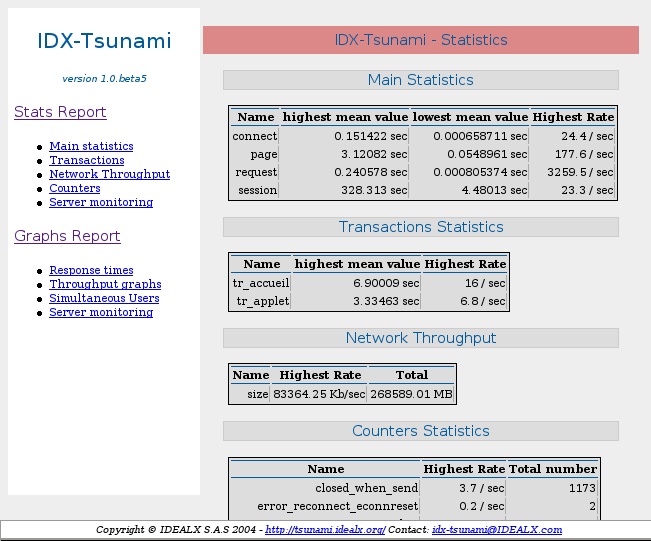
\includegraphics[width=0.6\linewidth]{tsunami-report}
    \end{center}
      \caption{Report}
    \label{fig:report}
\end{figure}

\subsection{Graphical overview}


\begin{figure}[htb]
  \begin{center}
    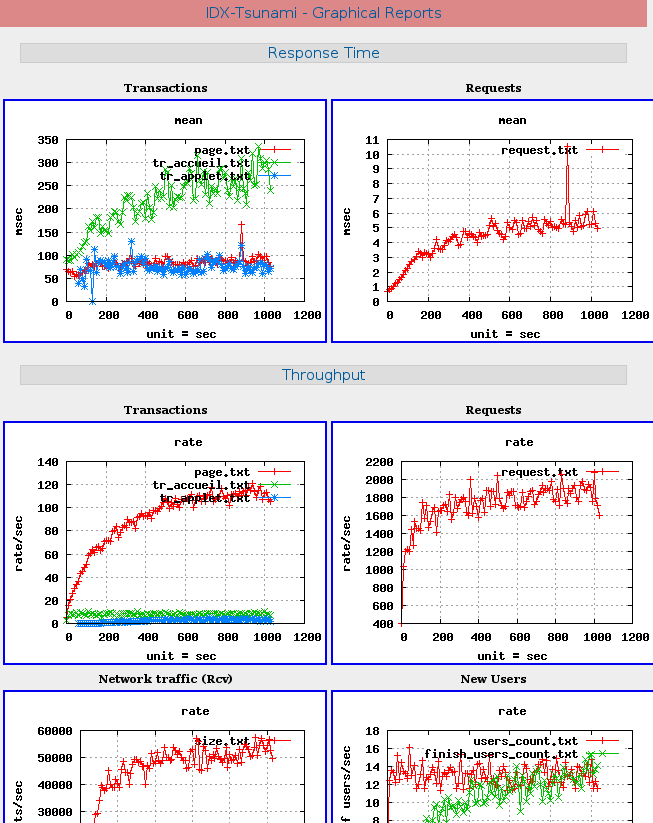
\includegraphics[width=0.6\linewidth]{tsunami-graph}
    \end{center}
      \caption{Graphical output}
    \label{fig:graph}
\end{figure}

%\section{Roadmap}

%FIXME

\section{References}

\begin{itemize}
\item \program{IDX-Tsunami} home page: \url{http://tsunami.idealx.org/}
\item \program{IDX-Tsunami} description (French)\footnote{\url{http://www.erlang-projects.org/Members/mremond/events/dossier_de_presentat/block_10766817551485/file}}
\item Erlang web site \url{http://www.erlang.org/}
\item Erlang programmation, Micka�l R�mond, Editions Eyrolles, 2003
  \footnote{\url{http://www.editions-eyrolles.com/php.accueil/Ouvrages/ouvrage.php3?ouv_ean13=9782212110791}}
\item \emph{Making reliable system in presence of software errors}, Doctoral Thesis,
Joe Armstrong, Stockholm, 2003 \footnote{\url{http://www.sics.se/~joe/thesis/armstrong_thesis_2003.pdf}}
\end{itemize}

\section{Acknowledgments}

The first version of this document was based on a talk given by Mickael
R�mond\footnote{\email{mickael.remond@erlang-fr.org}} during an Object
Web benchmarking workshop in April 2004 (more info at
\url{http://jmob.objectweb.org/}).


\begin{appendix}

\section{Frequently Asked Questions}

\subsection{IDX-tsunami crash when I start it }

Does your Erlang system has ssl support enabled ?

to test it:
\begin{Verbatim}
  > erl
  Eshell V5.2  (abort with ^G)
  1> ssl:start()
  you should see 'ok' 
\end{Verbatim}

\subsection{IDX-tsunami still doesn't start ...}

Most of the time, when a crash happened at startup without any traffic  
generated, the problem arise because the main Erlang controller node cannot  
create a "slave" Erlang virtual machine. The message looks like:

\begin{Verbatim}
===============================================
=ERROR REPORT==== 4-May-2004::22:38:26 ===
** Generic server ts_config_server terminating
** Last message in was {'$gen_cast',{newbeam,myshortname,[]}}
** When Server state == {state,{config,
                                     undefined,
                                     5,
                                     full,
                                     undefined,
                                     [{client,
                                          "myshortname",
                                          2.00000,
                                          5,
                                          [{10,68,133,140}]}],
                                     {server,"foo.net",80,gen_tcp},
                                     [],
                                     [{arrivalphase,
                                          1,
                                          60,
                                          undefined,
                                          undefined,
                                          5.00000e-5,
                                          infinity}],
                                     undefined,
                                     [{session,
                                          1,
                                          100,
                                          ts_http,
                                          parse,
                                          true,
                                          undefined}],
                                     14,
                                     3,
                                     7,
                                     6,
                                     "negociate"},
  "/home/username/.idx-tsunami/log/20040204-18:32",
                               undefined,
                               0,
                               undefined,
                               2.00000}
** Reason for termination ==
** {{badmatch,{error,timeout}},
    [{ts_config_server,handle_cast,2},
     {gen_server,handle_msg,6},
     {proc_lib,init_p,5}]}
\end{Verbatim} 
%%%$

IDX-Tsunami launches a new erl virtual machine to do the actual
injection even when you have only one machine in the injection
cluster. This is because it need to by-pass some limit with the number
of open socket from a single process (1024 most of the time). The idea
is to have several system processes (Erl beam) that can handle only a
small part of the network connection from the given computer. When the
\varname{maxclient} limit (simultaneous) is reach, a new Erlang beam is launched
and the newest connection can be handle by the new beam).

The problem is that the Erlang slave module cannot start a local slave
node. It tries to start it with the short node name
\varname{"myshortname"} (\command{erl -sname myshortname}).
 If this fails the injection process cannot
start. Most of the time, adding the short name with the correct IP
address in the \file{/etc/hosts} file is sufficient to make it work.

Note that you do not need to use the 127.0.0.1 address in the config file.  
It will not work if you use it as the injection interface. The shortname  
of your client machine should not refer to this address.

\strong{New in 1.1.0}: If you don't use the distributed feature of
Tsunami and have trouble to start a remote beam on a local machine,
you can set the \varname{'use_controller_vm'} attribute to true, for ex.:

\begin{Verbatim}
  <client host="mymachine" use_controller_vm="true">
\end{Verbatim}

\subsection{IDX-tsunami still crash/fails  when I start it !}
First look at the log file
\file{~/.idx-tsunami/log/XXX/tsunami_controller@yourhostname'} to see
if there is a problem. 

If you see nothing wrong, you can compile \program{idx-tsunami} with full
debugging: recompile with \command{make debug} , and
don't forget to set the loglevel to "debug" in the XML file.

To start the debugger or see what happen, start \program{IDX-Tsunami} with the
\userinput{debug} argument instead of \userinput{start}. You will have
an erlang shell on the \varname{tsunami\_controller} node. Use
\command{toolbar:start().} to launch the graphical tools provided by
Erlang.
\subsection{What is the format of the stats file idx-tsunami.log ?}

\begin{Verbatim}
# stats: dump at 1083694995
stats: users 11 11
stats: request 41 1.03289 0.125108 1.59802 0.901978
stats: connect 41 0.220170 6.67110e-2 0.494019 0.171997
stats: users_count 11 11
stats: page 24 6.80416 17.2794 80.4609 0.958984
stats: size 26818 26818
stats: 404 7 7
stats: 200 20 20
# stats: dump at 1083695005
stats: users 21 21
stats: request 113 1.03980 0.110650 1.59802 0.791016
stats: connect 118 0.197619 4.26037e-2 0.494019 0.163940
stats: users_count 10 21
stats: page 52 2.72266 1.74204 80.4609 0.791016
stats: size 78060 104878
stats: 404 15 22
stats: 200 51 71
 ...
\end{Verbatim}

 the format is, for \varname{request}, \varname{page}, \varname{session}:
 
 \texttt{ \# stats:'name' count(during the last 10sec), mean, stdvar,
   max, min}

 or for HTTP returns code, size ...

\texttt{ \# stats:'name' count(during the last 10sec), totalcount(since the beginning)}

\subsection{How can i specify the number of concurrent users ?}

You can't. But it's on purpose: the load generated by
\program{IDX-Tsunami} is dependent on the arrival time between new
clients. Indeed, once a client has finished his session in
\program{idx-tsunami}, it stops. So the number of concurrent users is
a function of the arrival rate and the mean session duration.

For example, if your web site has $1000$ visits/hour, the arrival rate
is $1000/3600 = 0.2778$ visits/second. If you want to simulate the same
load, set the inter-arrival time is to $1/0.27778 = 3.6 sec$ (\texttt{<users
interarrival="3.6" unit="second">} in the \varname{arrivalphase} node in the
XML config file).

\subsection{SNMP monitoring doesn't work ?!}

SNMP currently doesn't work with erlang R10B and up. Use erlang R9C-2 if you
need SNMP.

There is a small bug in the \file{snmp\_mgr} module in old Erlang
release (R9C-0). You have to apply this patch to make it
work. This is fixed in erlang R9C-1 and up.


\begin{Verbatim}
--- lib/snmp-3.4/src/snmp_mgr.erl.orig  2004-03-22 15:21:59.000000000 +0100
+++ lib/snmp-3.4/src/snmp_mgr.erl       2004-03-22 15:23:46.000000000 +0100
@@ -296,6 +296,10 @@
     end;
 is_options_ok([{recbuf,Sz}|Opts]) when 0 < Sz, Sz =< 65535 ->
     is_options_ok(Opts);
+is_options_ok([{receive_type, msg}|Opts]) ->
+    is_options_ok(Opts);
+is_options_ok([{receive_type, pdu}|Opts]) ->
+    is_options_ok(Opts);
 is_options_ok([InvOpt|_]) ->
     {error,{invalid_option,InvOpt}};
 is_options_ok([]) -> true.
\end{Verbatim}

\end{appendix}

\end{document}


%%% for AucTex/Emacs : 
%%% Local Variables: 
%%% eval:(setenv "TEXINPUTS" ":.:~/cvs/projetdoc//common/styles:./images:./figures:")
%%% mode: latex
%%% End: 
